% GENERATED by build_tex.py (anonymous: commit hashes replaced by labels, see commitmap.json)
\section{Supplementary figures}\label{app:supp}


\begin{figure}[htbp]
  \centering
  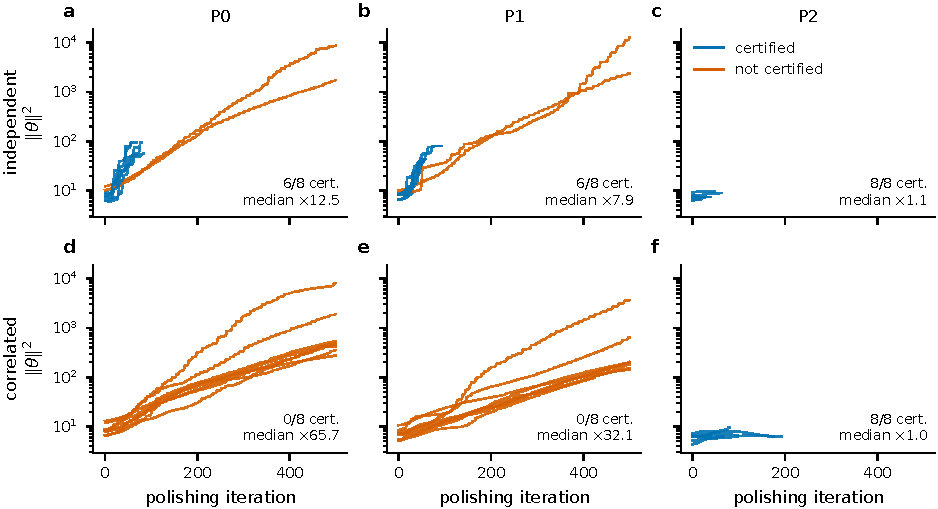
\includegraphics[width=\linewidth]{fig2_synthetic.pdf}
  % CAPTION-DRAFT: review (numbers from paper2/figures/fig2_synthetic.json)
  \caption{Synthetic $2\times3$ study: $\|\theta\|^2$ over exact-Hessian trust-region polishing iterations (log scale), one line per seed, coloured certified (blue) or not certified (vermillion). Rows: independent and correlated inputs; columns: P0, P1, P2. Per panel, certified seeds and median growth (polished over early-stopped): independent P0: 6/8 certified, $\times$12.5; independent P1: 6/8 certified, $\times$7.9; independent P2: 8/8 certified, $\times$1.1; correlated P0: 0/8 certified, $\times$65.7; correlated P1: 0/8 certified, $\times$32.1; correlated P2: 8/8 certified, $\times$1.0.}
  \label{fig:synthetic}
\end{figure}


\begin{figure}[htbp]
  \centering
  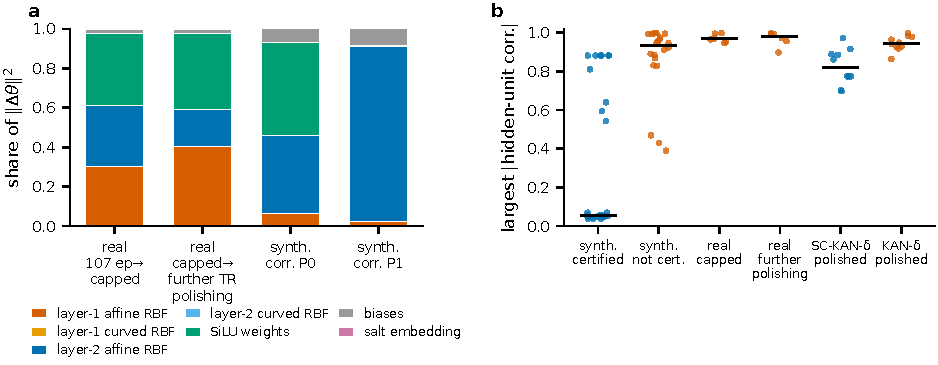
\includegraphics[width=\linewidth]{fig3_where.pdf}
  % CAPTION-DRAFT: review (numbers from paper2/figures/fig3_where.json)
  \caption{Where the runaway lives. \textbf{(a)} Mean share of $\|\Delta\theta\|^2$ by parameter block. Real data, 107 epochs$\to$capped: layer-1 affine RBF 0.30, layer-2 affine RBF 0.31, SiLU weights 0.37; capped$\to$further trust-region polishing: 0.40, 0.19, 0.38; synthetic correlated P0: layer-2 affine RBF 0.39, SiLU weights 0.47; correlated P1: layer-2 affine RBF 0.89. The real-data split was evaluated post hoc from archived weights (Appendix~\ref{app:repro}). \textbf{(b)} Largest absolute correlation between hidden-unit activations on the training rows, median: synthetic, certified 0.054 ($n=28$); synthetic, not certified 0.935 ($n=20$); real, capped 0.968 ($n=6$); real, further polishing 0.983 ($n=6$); SC-KAN-$\delta$ polished 0.818 ($n=10$); KAN-$\delta$ polished 0.946 ($n=10$). Blue: certified; vermillion: not certified or runaway.}
  \label{fig:where}
\end{figure}


\begin{figure}[htbp]
  \centering
  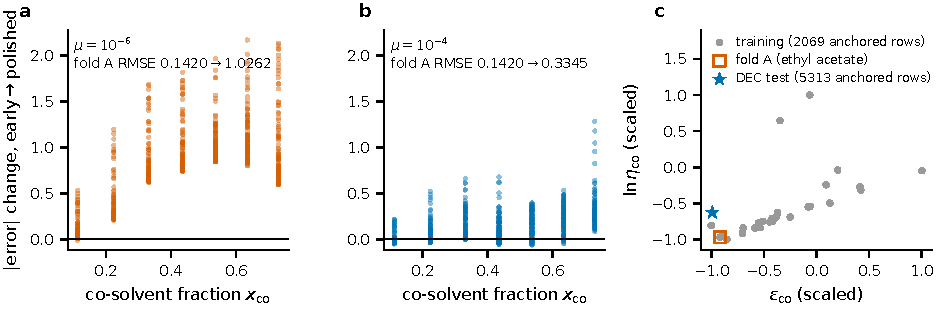
\includegraphics[width=\linewidth]{fig4_applicability.pdf}
  % CAPTION-DRAFT: review (numbers from paper2/figures/fig4_applicability.json)
  \caption{Applicability (descriptive; analysis plan committed before computing). \textbf{(a, b)} Fold A (ethyl acetate held out, 635 rows): change in each row's absolute error from the early-stopped 5-seed ensemble to the polished ensemble, against the co-solvent fraction $x_{\mathrm{co}}$ (7 distinct values); fold A RMSE 0.1420$\to$1.0262 at $\mu = 10^{-6}$ (a) and 0.1420$\to$0.3345 at $\mu = 10^{-4}$ (b). Per-row values are evaluated post hoc from SHA-verified archived weights, with the logged RMSEs reproduced (Appendix~\ref{app:repro}). \textbf{(c)} Co-solvent descriptors $\varepsilon_{\mathrm{co}}$ and $\ln\eta_{\mathrm{co}}$ in the committed min--max scaling: the 2069 anchored training rows (30 distinct points), fold A's co-solvent (off-pattern distance 0.047) and the 5313 anchored DEC test rows (0.334); each held-out set occupies a single point.}
  \label{fig:applicability}
\end{figure}


\begin{figure}[htbp]
  \centering
  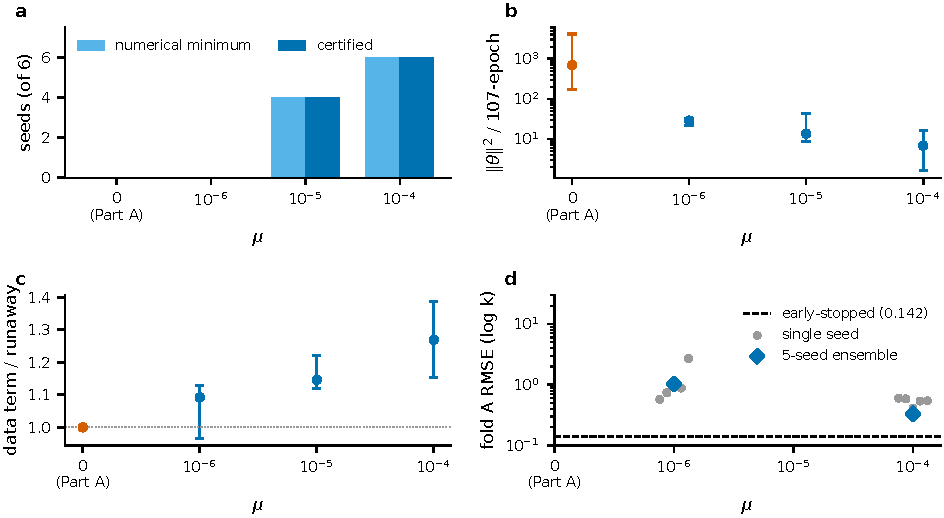
\includegraphics[width=\linewidth]{fig8_dose_response.pdf}
  % CAPTION-DRAFT: review (numbers from paper2/figures/fig8_dose_response.json)
  \caption{Real-data dose-response in the null-space weight $\mu$ (6 KAN-$\delta$ seeds; $\mu = 0$: polished without a null-space penalty). \textbf{(a)} Seeds at a numerical minimum (all of them certified): $\mu = 0$, 0 of 6; $10^{-6}$, 0 of 6; $10^{-5}$, 4 of 6; $10^{-4}$, 6 of 6. \textbf{(b)} $\|\theta\|^2$ relative to the 107-epoch state, median (range): $\mu = 0$, 690 (170--4146); $10^{-6}$, 29 (21--31); $10^{-5}$, 14 (9--43); $10^{-4}$, 7 (2--16). \textbf{(c)} Training data term relative to the runaway, median: $10^{-6}$, 1.092; $10^{-5}$, 1.146; $10^{-4}$, 1.269. \textbf{(d)} Fold A RMSE: early-stopped 0.142 (dashed line); polished 5-seed ensemble 1.026 at $\mu = 10^{-6}$ and 0.334 at $\mu = 10^{-4}$; grey points are single seeds.}
  \label{fig:dose}
\end{figure}


\begin{figure}[h]
  \centering
  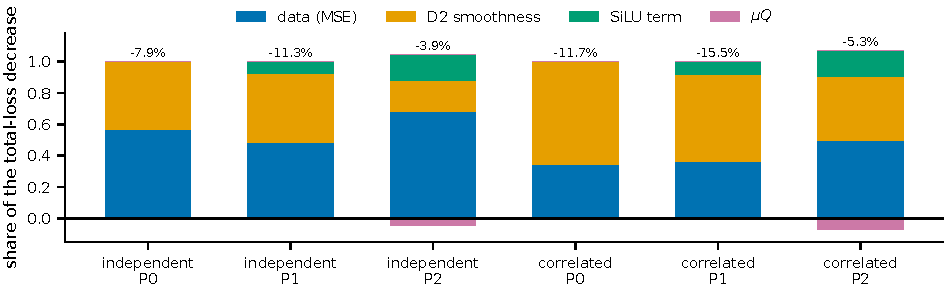
\includegraphics[width=\linewidth]{figS1_lossdecomp.pdf}
  % CAPTION-DRAFT: review (numbers from paper2/figures/figS1_lossdecomp.json)
  \caption{Post hoc loss decomposition (synthetic, early$\to$polished): share of the total-loss decrease from each term, pooled over the 8 seeds of each cell. independent P0: data 0.57, D2 0.43 (median total change -7.9\%); independent P1: data 0.49, D2 0.44 (median total change -11.3\%); independent P2: data 0.68, D2 0.20 (median total change -3.9\%); correlated P0: data 0.35, D2 0.65 (median total change -11.7\%); correlated P1: data 0.37, D2 0.55 (median total change -15.5\%); correlated P2: data 0.50, D2 0.40 (median total change -5.3\%).}
  \label{fig:S1}
\end{figure}


\begin{figure}[h]
  \centering
  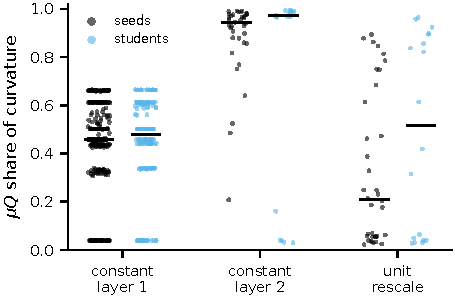
\includegraphics[width=0.5\linewidth]{figS2_gaugecheck.pdf}
  % CAPTION-DRAFT: review (numbers from paper2/figures/figS2_gaugecheck.json)
  \caption{Post hoc gauge check at the $\mu = 10^{-4}$ certified minima: share of the curvature along each least-squares gauge direction contributed by $\mu Q$. Medians: constant shift in layer 1, real-data seeds 0.46 ($n = 288$); constant shift in layer 1, students (trained on a frozen teacher) 0.48 ($n = 144$); constant shift in layer 2, real-data seeds 0.94 ($n = 36$); constant shift in layer 2, students 0.97 ($n = 18$); unit rescaling, real-data seeds 0.21 ($n = 36$); unit rescaling, students 0.52 ($n = 18$).}
  \label{fig:S2}
\end{figure}


\begin{figure}[h]
  \centering
  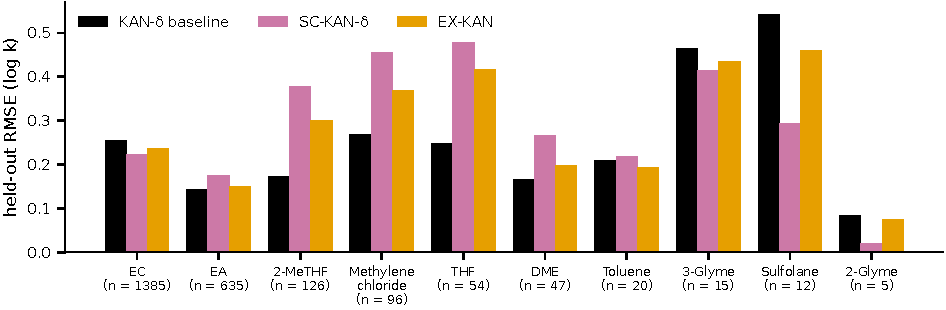
\includegraphics[width=\linewidth]{figS3_loco.pdf}
  % CAPTION-DRAFT: review (numbers from paper2/figures/figS3_loco.json)
  \caption{Leave-one-co-solvent-out RMSE per fold (5-seed ensembles, early state) for the KAN-$\delta$ baseline, SC-KAN-$\delta$ and EX-KAN. Unweighted means: KAN-$\delta$ baseline 0.2554; SC-KAN-$\delta$ 0.2923; EX-KAN 0.2834. The EA fold uses the fold A rows.}
  \label{fig:S3}
\end{figure}

\clearpage  % flush Appendix E's figures before Appendix F